\documentclass[UTF8]{ctexart}
\usepackage{listings}
\usepackage{booktabs}  
\usepackage{geometry}  
\usepackage{graphicx} 
\usepackage{xcolor}
\usepackage{float}
\usepackage{array}
\usepackage{enumitem}
\usepackage{amsmath,amssymb,bm}
\usepackage[version=4]{mhchem}
\usepackage{siunitx}
\usepackage{tikz}
\usepackage{pgfplots}
\pgfplotsset{compat=1.18}
% 移除biblatex,使用natbib进行引用管理
\usepackage[numbers,sort&compress]{natbib}
\usepackage[colorlinks=true]{hyperref} 
\usepackage{xurl} 
\usepackage{url}
\hypersetup{
    colorlinks = true,
    linkcolor = blue,
    citecolor = blue,
    urlcolor = blue,
    pdftitle = {CFD Final Project},
    pdfsubject = {Computational Fluid Dynamics},
    pdfauthor = {朱林}
}

\pgfplotsset{compat=1.18}
\graphicspath{{figure/}}
\geometry{a4paper, left=2.5cm, right=2.5cm, top=2.5cm, bottom=2.5cm}
\definecolor{codegreen}{rgb}{0,0.6,0}
\definecolor{codegray}{rgb}{0.5,0.5,0.5}
\definecolor{codepurple}{rgb}{0.58,0,0.82}
\lstset{
    basicstyle=\ttfamily\footnotesize,
    breaklines=true,
    frame=single,
    numbers=left,
    numberstyle=\tiny\color{codegray},
    keywordstyle=\color{blue},
    commentstyle=\color{codegreen},
    stringstyle=\color{codepurple},
    showstringspaces=false
}



\begin{document}
\title{计算流体力学期末大作业}
\author{朱林-2200011028}
\date{\today}
\maketitle

\section{数理算法原理}
\subsection{问题描述}
\subsubsection{物理情形}
Sod激波管问题是一个一维理想气体流动问题:无限长管道中,初始时刻($t=0$)在$x=0$处有一薄膜分隔两侧气体:
\begin{itemize}
    \item 左侧($x<0$): 高压区,状态为$(\rho_L, u_L, p_L)$
    \item 右侧($x>0$): 低压区,状态为$(\rho_R, u_R, p_R)$
\end{itemize}

薄膜在$t=0^+$时刻瞬时破裂,两侧气体开始相互作用,产生复杂的波系结构。

\subsubsection{标准初始条件}
采用以下无量纲初始条件:
\begin{align*}
\text{左侧:} & \quad \rho_L = 1.0,  u_L = 0.0,  p_L = 1.0 \\
\text{右侧:} & \quad \rho_R = 0.125,  u_R = 0.0,  p_R = 0.1
\end{align*}

\subsection{控制方程}
流动由一维欧拉方程描述:
\begin{align}
&\frac{\partial \mathbf{U}}{\partial t} + \frac{\partial f(\mathbf{U})}{\partial x} = 0 \\
&\mathbf{U} = \begin{bmatrix} \rho \\ \rho u \\ E \end{bmatrix}, \quad
f(\mathbf{U}) = \begin{bmatrix} \rho u \\ \rho u^2 + p \\ u(E + p) \end{bmatrix}
\end{align}
其中总能密度$E = \rho e = \rho (C_v T + \frac{1}{2}u^2)$。

\subsection{Riemann问题精确解}
\subsubsection{波系结构}
根据空气动力学知识,该 Sod 激波管中可能出现三种波:
\begin{itemize}
    \item 激波:流体密度、速度、压力均发生突变,满足 Rankine-Hugoniot (R-H) 关系式。
    \item 接触间断:流体仅密度发生突变,速度与压力不变。
    \item 膨胀波(稀疏波):一种等熵波,其内部物理量连续、光滑,头、尾物理量连续但导数不连续(弱间断),且 Riemann 不变量不变。
\end{itemize}
对于一维sod激波管问题,薄膜破裂后将形成向左传播的膨胀波、向右传播的接触间断和激波,如图\ref{fig:wave_structure_1}。
这些波将流场划分为五个特征区域(如图\ref{fig:wave_structure_2}所示\footnote{url:https://blog.csdn.net/Nidebear/article/details/109300513}):
\begin{figure}[H]
    \centering
    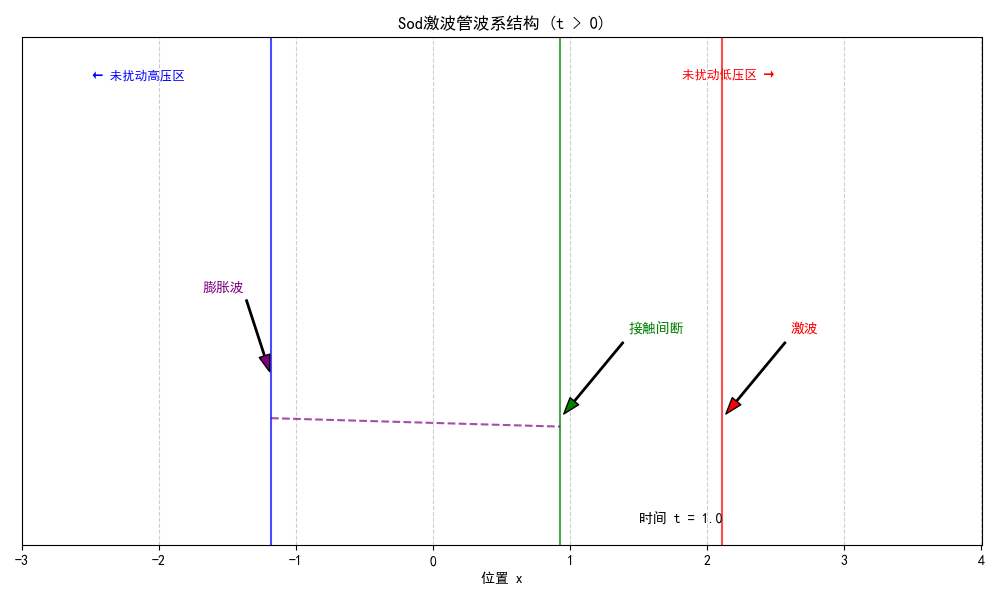
\includegraphics[width=0.8\textwidth]{wave_structure_1.png}
    \caption{Sod激波管典型波系结构(t>0)}
    \label{fig:wave_structure_1}
\end{figure}
\begin{figure}[H]
    \centering
    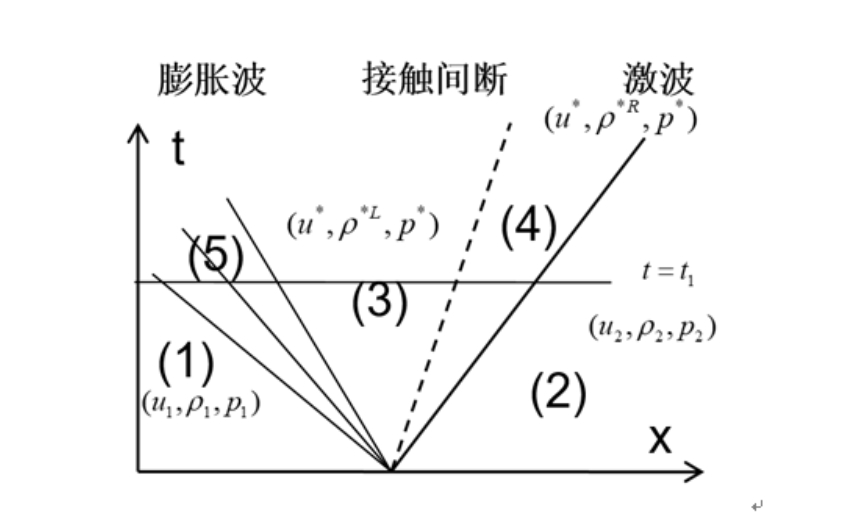
\includegraphics[width=0.8\textwidth]{wave_structure_2.png}
    \caption{Sod激波管典型波系结构}
    \label{fig:wave_structure_2}
\end{figure}
\begin{itemize}
    \item \textbf{区域1} 未扰动的左侧高压区,保持初始状态 $(\rho_L, u_L, p_L)$
    \item \textbf{区域2} 未扰动的右侧低压区,保持初始状态 $(\rho_R, u_R, p_R)$
    \item \textbf{区域3} 膨胀波后,状态为 $(\rho_2, u^*, p^*)$
    \item \textbf{区域4} 接触间断与激波间均匀区,状态为 $(\rho_3, u^*, p^*)$
    \item \textbf{区域5} 膨胀波内部
\end{itemize}

其中 $u^*$ 和 $p^*$ 为接触间断处的速度和压力,各波位置随时间线性变化:
$$x_{\text{left}} = -c_L t, \quad x_{\text{contact}} = u^* t, \quad x_{\text{shock}} = W_s t$$
$W_s$ 为激波传播速度,$c_L = \sqrt{\gamma p_L/\rho_L}$ 为左侧声速。

\subsubsection{解析解表达式}
解析解通过求解以下方程组获得:
\paragraph{1-3 两区, 等熵关系式}
\begin{equation}
    \frac{p^{*}}{\left(\rho^{* L}\right)^{\gamma}}=\frac{p_{1}}{\left(\rho_{1}\right)^{\gamma}}
\end{equation}
\begin{equation}
u_{1}+\frac{2 c_{1}}{\gamma-1}=u^{*}+\frac{2 c^{L}}{\gamma-1}
\end{equation}
其中, $c^{L}=\sqrt{\gamma p^{*} / \rho^{* L}}$。
\paragraph{2-4 两区, 激波 R-H 关系式}
\begin{equation}
\left\{\begin{array}{l}\rho_{2}\left(u_{2}-Z_{2}\right)=\rho^{* R}\left(u^{*}-Z_{2}\right) \\\rho_{2} u_{2}\left(u_{2}-Z_{2}\right)+p_{2}=\rho^{* R} u^{*}\left(u^{*}-Z_{2}\right)+p^{*} \\E_{2}\left(u_{2}-Z_{2}\right)+u_{2} p_{2}=E^{* R}\left(u^{*}-Z_{2}\right)+p^{*} u^{*}\end{array}\right.
\end{equation}
以上变量说明从略。综上 5 个方程、 5 个未知数,故方程组可解,求解方法为联立以上两个方程组,解出 3、4 区内速度对压力的依赖关系,有

$$u^{*}=u_{1}-f(p^{*},p_{1},\rho_{1})$$

其中,满足 
\begin{equation}
f(p^{*},p_{i},\rho_{i})=\frac{2c_{i}}{\gamma-1}\left[\left(\frac{p^{*}}{p_{i}}\right)^{\frac{\gamma-1}{2\gamma}}-1\right]
\end{equation}
注意到,激波、膨胀波前后速度-压力的依赖关系可写成统一的形式:

左波(激波或膨胀波)

$$u^{*}=u_{1}-f(p^{*},p_{1},\rho_{1})$$

右波(激波或膨胀波)

$$u^{*}=u_{2}+f(p^{*},p_{2},\rho_{2})$$

以上 $u^{*},p^{*}$ 表示 3、4 区内的速度与压力,其中

\begin{equation}
f(p^{*},p_{i},\rho_{i})=\left\{\begin{array}{ll}\frac{p^{*}-p_{i}}{\rho_{i}c_{i}\left[\frac{\gamma+1}{2\gamma}\left(\frac{p^{*}}{p_{i}}\right)+\frac{\gamma-1}{2\gamma}\right]^{1/2}}, & p^{*}>p_{i}\\\frac{2c_{i}}{\gamma-1}\left[\left(\frac{p^{*}}{p_{i}}\right)^{\frac{\gamma-1}{2\gamma}}-1\right], & p^{*}<p_{i}\end{array}\right.
\end{equation}

求解上式可得到 3、4 区内的压力,然后可以解得速度和密度。
\paragraph{膨胀波内部}

对于膨胀波内部物理量的计算,首先由波头传播速度$u_1-c_1$与波尾传播速度$u^*-c^{*L}$
可计算膨胀波的范围。在膨胀波区内,利用特征相容关系和等熵关系计算物理量,可利
用简单波的特性来简化计算。以下直接给出各个物理量的计算表达式:
$$\begin{aligned}&c(t,x)=\frac{\gamma-1}{\gamma+1}\left(u_{1}-\frac{x}{t}\right)+\frac{2}{\gamma+1}c_{1}\\&u(x,t)=c+x/t\\&p=p_{1}\:(c/c_{1})^{2\gamma/\gamma-1}\\&\rho=\gamma p/c^{2}\end{aligned}$$
综上所述,一维 Riemann 问题的精确解的求解思路与方程介绍完毕。本文 Sod 激波管参考
精确解程序来自于 GitLab 上的项目 simple shock tube calculator \cite{sodcal2025}。

\subsection{数值计算方法}
% 补充边界条件说明
\subsubsection{计算域与网格}

计算域默认设置为 $x \in [-5, 5]$,时间计算域为 $t \in [0, 2.0]$,该范围足以捕捉Sod问题中激波、接触间断和膨胀波的完整演化过程。空间离散采用均匀网格划分,网格间距 $\Delta x$ 由计算域长度和网格数动态确定。时间步长 $\Delta t$ 根据CFL条件自适应调整:

\begin{equation}
\Delta t = \text{CFL} \cdot \frac{\Delta x}{\max(|u| + c)}
\end{equation}

边界条件采用无反射处理:
\begin{align*}
U_0 &= U_1 \\
U_{N+1} &= U_N
\end{align*}
此边界处理可有效抑制数值反射,确保波系在计算域内自由传播。网格收敛性研究表明,接触间断分辨率对网格依赖性显著,需足够细密的网格才能准确捕捉密度突变特征。

\subsubsection{激波捕捉格式}
\paragraph{TVD格式(Minmod限制器)}

总变差定义:
\begin{equation}
TV(U^n) = \sum_{i=-\infty}^{\infty} |U_{i+1}^n - U_i^n|
\end{equation}
TVD条件:
\begin{equation}
TV(U^{n+1}) \leq TV(U^n)
\end{equation}
通量限制器格式:
\begin{equation}
F_{i+\frac{1}{2}} = F_i + \frac{1}{2} \phi(r_i) (F_{i+1} - F_i)
\end{equation}
梯度比:
\begin{equation}
r_i = \frac{U_i - U_{i-1}}{U_{i+1} - U_i}
\end{equation}
Minmod限制器函数:
\begin{equation}
\phi(r) = \text{minmod}(1, r) = 
\begin{cases} 
0 & r \leq 0 \\
r & 0 < r < 1 \\
1 & r \geq 1 
\end{cases}
\end{equation}
性质:
\begin{itemize}
\item 满足二阶精度条件:$\phi(1)=1$
\item 满足TVD条件:$0 \leq \phi(r) \leq \min(2,2r)$
\item 在间断处退化为单调的一阶格式
\end{itemize}

\paragraph{群速度控制(GVC)格式}

通量修正方程:
\begin{equation}
\mathbf{F}^{GVC} = \mathbf{F}^{base} + \epsilon \Delta x^3 \frac{\partial^3 \mathbf{U}}{\partial x^3}
\end{equation}
三阶导数离散:
\begin{equation}
\left.\frac{\partial^3 U}{\partial x^3}\right|_i \approx \frac{-U_{i-2} + 2U_{i-1} - 2U_{i+1} + U_{i+2}}{2\Delta x^3}
\end{equation}
自适应控制系数:
\begin{equation}
\epsilon = C \cdot |u \pm c|, \quad C \in [0.1, 0.5]
\end{equation}
修正后群速度:
\begin{equation}
v_g^{num} = v_g^{exact} - 4\epsilon k^2 \Delta x^2
\end{equation}

\paragraph{WENO格式}

\textbf{基本框架}

\begin{enumerate}
\item 选择模板:$S_0=\{I_{i-2},I_{i-1},I_i\}$, $S_1=\{I_{i-1},I_i,I_{i+1}\}$, $S_2=\{I_i,I_{i+1},I_{i+2}\}$
\item 重构多项式:
\begin{align}
p_0(x) &= \frac{1}{3}U_{i-2} - \frac{7}{6}U_{i-1} + \frac{11}{6}U_i \\
p_1(x) &= -\frac{1}{6}U_{i-1} + \frac{5}{6}U_i + \frac{1}{3}U_{i+1} \\
p_2(x) &= \frac{1}{3}U_i + \frac{5}{6}U_{i+1} - \frac{1}{6}U_{i+2}
\end{align}
\end{enumerate}

\textbf{WENO-JS}
光滑指示器:
\begin{align}
\beta_k &= \sum_{l=1}^{2} \Delta x^{2l-1} \int_{x_{i-1/2}}^{x_{i+1/2}} \left( \frac{d^l p_k(x)}{dx^l} \right)^2 dx \\
\beta_0 &= \frac{13}{12}(U_{i-2}-2U_{i-1}+U_i)^2 + \frac{1}{4}(U_{i-2}-4U_{i-1}+3U_i)^2 \\
\beta_1 &= \frac{13}{12}(U_{i-1}-2U_i+U_{i+1})^2 + \frac{1}{4}(U_{i-1}-U_{i+1})^2 \\
\beta_2 &= \frac{13}{12}(U_i-2U_{i+1}+U_{i+2})^2 + \frac{1}{4}(3U_i-4U_{i+1}+U_{i+2})^2
\end{align}
非线性权重:
\begin{align}
\alpha_k &= \frac{d_k}{(\beta_k + \varepsilon)^p}, \quad \omega_k = \frac{\alpha_k}{\sum_{m=0}^{2} \alpha_m} \\
d_0 &= 0.3, \quad d_1 = 0.6, \quad d_2 = 0.1 \\
\varepsilon &= 10^{-6}, \quad p = 2
\end{align}

\textbf{WENO-Z}

改进权重:
\begin{align}
\tau_5 &= |\beta_0 - \beta_2| \\
\alpha_k^Z &= d_k \left( 1 + \frac{\tau_5}{\beta_k + \varepsilon} \right) \\
\omega_k^Z &= \frac{\alpha_k^Z}{\sum_{m=0}^{2} \alpha_m^Z}
\end{align}
优势:光滑区$\omega_k \to d_k$,收敛阶$\mathcal{O}(\Delta x^5)$

\subsubsection{通量处理方法}

\paragraph{通量矢量分裂(FVS)}

\textbf{Steger-Warming分裂}

\begin{align}
\mathbf{F} &= \mathbf{F}^+ + \mathbf{F}^- = \mathbf{R}\mathbf{\Lambda}^+\mathbf{R}^{-1}\mathbf{U} + \mathbf{R}\mathbf{\Lambda}^-\mathbf{R}^{-1}\mathbf{U} \\
\lambda^\pm &= \frac{\lambda \pm |\lambda|}{2}
\end{align}
一维欧拉方程形式:
\begin{equation}
\mathbf{f}^{\pm} = \frac{\rho}{2\gamma} \begin{bmatrix}
(\gamma-1)\lambda_1^\pm + \lambda_3^\pm + \lambda_5^\pm \\
2(\gamma-1)\lambda_1^\pm u + \lambda_3^\pm (u+c) + \lambda_5^\pm (u-c) \\
(\gamma-1)\lambda_1^\pm u^2 + \frac{1}{2}\lambda_3^\pm (u+c)^2 + \frac{1}{2}\lambda_5^\pm (u-c)^2 + \frac{3-\gamma}{2(\gamma-1)}(\lambda_3^\pm + \lambda_5^\pm)c^2
\end{bmatrix}
\end{equation}

\textbf{Van Leer分裂}

质量通量分裂:
\begin{equation}
(\rho u)^\pm = \pm \frac{\rho c}{4} (M \pm 1)^2, \quad |M| \leq 1
\end{equation}
通量函数:
\begin{equation}
\mathbf{F}^\pm = \begin{bmatrix}
(\rho u)^\pm \\
(\rho u)^\pm \left[ \frac{(\gamma-1)u \pm 2c}{\gamma} \right] \\
(\rho u)^\pm \left[ \frac{ \left( (\gamma-1)u \pm 2c \right)^2 }{2(\gamma^2-1)} \right]
\end{bmatrix}
\end{equation}

\textbf{AUSM分裂}

通量分解:
\begin{equation}
\mathbf{F} = \dot{m}\mathbf{\Phi} + \mathbf{P}, \quad \mathbf{\Phi} = [1, u, H]^T
\end{equation}
界面通量:
\begin{equation}
\mathbf{f}_{1/2} = \dot{m}_{1/2}\mathbf{\Phi}_{L/R} + \mathbf{P}_{1/2}
\end{equation}
质量流量:
\begin{equation}
\dot{m}_{1/2} = c_{1/2} \begin{cases}
M_{1/2} \rho_L & M_{1/2} > 0 \\
M_{1/2} \rho_R & \text{其他}
\end{cases}, \quad M_{1/2} = M_L^+ + M_R^-
\end{equation}

\textbf{Lax-Friedrichs分裂}
\begin{equation}
\mathbf{F}^\pm = \frac{1}{2} (\mathbf{F} \pm \alpha \mathbf{U}), \quad \alpha = \max|\lambda_i|
\end{equation}

\paragraph{通量差分分裂(FDS)}

\textbf{Roe方法}

Roe平均:
\begin{align}
\hat{\rho} &= \sqrt{\rho_L \rho_R} \\
\hat{u} &= \frac{\sqrt{\rho_L}u_L + \sqrt{\rho_R}u_R}{\sqrt{\rho_L} + \sqrt{\rho_R}} \\
\hat{H} &= \frac{\sqrt{\rho_L}H_L + \sqrt{\rho_R}H_R}{\sqrt{\rho_L} + \sqrt{\rho_R}}
\end{align}
通量计算:
\begin{equation}
\mathbf{f}_{1/2} = \frac{1}{2} \left( \mathbf{F}_L + \mathbf{F}_R \right) - \frac{1}{2} \sum_{k=1}^{3} |\hat{\lambda}_k| \hat{\alpha}_k \hat{\mathbf{r}}_k
\end{equation}

\textbf{HLL方法}

通量计算:
\begin{equation}
\mathbf{f}_{\text{HLL}} = \begin{cases} 
\mathbf{f}_L & S_L \geq 0 \\
\frac{S_R\mathbf{f}_L - S_L\mathbf{f}_R + S_LS_R(\mathbf{U}_R - \mathbf{U}_L)}{S_R - S_L} & S_L < 0 < S_R \\
\mathbf{f}_R & S_R \leq 0
\end{cases}
\end{equation}
波速估计:
\begin{equation}
S_L = \min(u_L - c_L, \tilde{u} - \tilde{c}), \quad S_R = \max(u_R + c_R, \tilde{u} + \tilde{c})
\end{equation}

\textbf{Lax-Wendroff方法}

二阶中心格式:
\begin{equation}
\mathbf{f}_{i+1/2} = \mathbf{f}\left( \mathbf{u}_{i+1/2}^{\text{LW}} \right)
\end{equation}
中间状态:
\begin{equation}
\mathbf{u}_{i+1/2}^{\text{LW}} = \frac{1}{2} (\mathbf{u}_i + \mathbf{u}_{i+1}) - \frac{\Delta t}{2\Delta x} (\mathbf{f}_{i+1} - \mathbf{f}_i)
\end{equation}

\subsubsection{时间推进格式}
三阶Runge-Kutta (SSP-RK3):
\begin{align}
\mathbf{U}^{(1)} &= \mathbf{U}^n + \Delta t \mathcal{L}(\mathbf{U}^n) \\
\mathbf{U}^{(2)} &= \frac{3}{4}\mathbf{U}^n + \frac{1}{4}\left[ \mathbf{U}^{(1)} + \Delta t \mathcal{L}(\mathbf{U}^{(1)}) \right] \\
\mathbf{U}^{n+1} &= \frac{1}{3}\mathbf{U}^n + \frac{2}{3}\left[ \mathbf{U}^{(2)} + \Delta t \mathcal{L}(\mathbf{U}^{(2)}) \right]
\end{align}
稳定性条件:
\begin{equation}
\text{CFL} = \max \left( |u| + c \right) \frac{\Delta t}{\Delta x} \leq 1.5
\end{equation}

\newpage
\section*{符号说明}
\begin{table}[h]
\centering
\begin{tabular}{c|l}
\hline
符号 & 物理意义 \\
\hline
$\rho$ & 密度 \\
$u$ & 速度 \\
$p$ & 压强 \\
$E$ & 总能 \\
$c$ & 声速 $c = \sqrt{\gamma p / \rho}$ \\
$H$ & 总焓 $H = (E + p)/\rho$ \\
$\gamma$ & 比热比 \\
$\mathbf{R},\mathbf{L}$ & 右/左特征向量矩阵 \\
$\lambda$ & 特征值 \\
$\Delta x$ & 空间步长 \\
$\Delta t$ & 时间步长 \\
\hline
\end{tabular}
\end{table}

\newpage
\section{代码生成与调试}
由于本次的代码量大,且要求复杂,所以编写代码的过程中严格遵循模块化思路,在编写之初就按照功能划分了多个模块,分别为:
\begin{itemize}
    \item \textbf{main.py}:主程序入口,负责整体流程控制
    \item \textbf{config.py}:配置模块,存储参数设置和初始条件
    \item \textbf{time\_integration.py}:时间积分模块,包含三阶Runge--Kutta方法实现
    \item \textbf{utils}:工具函数库,包含数据处理、可视化、调用精确解、边界条件处理等功能
    \item \textbf{initialization}: 初始条件模块,负责设置初始状态和网格划分
    \item \textbf{flux}: 通量计算模块,包含FVS、FDS等格式实现
    \item \textbf{schemes}: 数值格式模块,包含TVD、WENO等格式实现
\end{itemize}
对于每个模块,在编写完成后都进行了单元测试,确保各个模块功能正确。主程序通过调用这些模块实现整体流程控制。测试所用的程序在\textbf{test}目录下\footnote{如果希望运行测试程序,请将其放置到src目录下}
,包含了对各个模块的单元测试脚本。接下来我将按照编写的顺序对各个模块进行介绍。
\subsection{initialization}
在初始化模块下,我一共编写两个文件:一个是 \textbf{domain\_setup.py},用于设置计算域和网格划分;另一个是 \textbf{sod\_initial.py},用于设置初始条件。

在test目录中的\textbf{initialization\_test.py}中,我对这两个模块进行了单元测试,确保它们能够正确设置计算域和初始条件。
\subsection{utils}
在工具函数模块下,我编写了\textbf{boundary.py}、\textbf{exact\_solution.py}、\textbf{visualization.py}三个文件,同时还将来自GitLab\cite{sodcal2025}的代码\textbf{gitlab\_sod\_analytical.py}也放置于此模块下。
其中\textbf{boundary.py}实现了三种边界条件处理,\textbf{exact\_solution.py}在调用GitLab上的代码的基础上实现了Sod激波管问题的精确解计算,\textbf{visualization.py}实现了结果可视化功能。

在test目录中的\textbf{boundary\_test.py}、\textbf{exact\_solution\_test.py}和\textbf{visualization\_test.py}中,我对这些工具函数进行了单元测试,确保它们能够正确处理边界条件、计算精确解和可视化结果。
\subsection{flux}
在通量计算模块下,我编写了\textbf{flux\_fvs.py}和\textbf{flux\_fds.py}两个文件,分别实现了FVS和FDS格式的通量计算。
其中\textbf{flux\_fvs.py}实现了Steger-Warming、Van Leer、AUSM和Lax-Friedrichs四种通量分裂方法,\textbf{flux\_fds.py}实现了HLL、Roe和Lax-Wendroff三种通量差分分裂方法。
但是其中的Roe方法存在问题,我在尝试多次后仍然未能解决bug,所以在择时请勿使用Roe方法。
\subsection{schemes}
在数值格式模块下,我编写了\textbf{tvd.py}、 \textbf{weno.py}和\textbf{gvc.py}三个文件,分别实现了TVD格式、WENO格式和群速度控制格式。
其中\textbf{tvd.py}实现了Minmod限制器的TVD格式,\textbf{weno.py}实现了WENO-JS和WENO-Z格式,\textbf{gvc.py}实现了群速度控制格式。

在test目录中的\textbf{tvd\_fvs\_rk3\_test.py}中,我对于TVD、FVS和RK3格式进行了单元测试,确保在这一组合下能够正确计算Sod激波管问题的数值解。

在test目录中的\textbf{weno\_test.py}中,我对WENO格式进行了单元测试,确保其能够正确处理Sod激波管问题的数值解。

在test目录中的\textbf{gvc\_test.py}中,我对群速度控制格式进行了单元测试,确保其能够正确处理Sod激波管问题的数值解。

在test目录中的\textbf{fds\_test.py}中,我在使用TVD格式的基础上,测试了FDS格式的通量计算,确保其能够正确处理Sod激波管问题的数值解。
\subsection{time\_integration.py}
主目录下,我编写了\textbf{time\_integration.py},用于实现三阶Runge-Kutta时间积分方法和计算$\Delta t$。
\subsection{config.py}
在主目录下,我编写了\textbf{config.py},用于存储参数设置和初始条件。该文件包含了所有需要的参数,如计算域、网格划分、初始条件等。此外,在这个文件中,
用户可以自主选择使用的数值格式和通量计算方法。这样可以方便地进行参数调整和格式切换,而无需修改其他代码。
\subsection{main.py}
作为项目的主程序入口,\textbf{main.py}负责整体流程控制。它首先导入配置文件中的参数设置,然后调用各个模块实现Sod激波管问题的数值计算和可视化。

\subsection{使用方法}
在项目的 src 目录下,用户可以通过以下命令运行主程序:
\begin{verbatim}
    python main.py
\end{verbatim}
运行后,程序将自动执行以下步骤:
\begin{enumerate}           
    \item 导入配置文件中的参数设置
    \item 调用初始化模块设置计算域和初始条件
    \item 调用工具函数模块处理边界条件和计算精确解
    \item 调用通量计算模块计算通量
    \item 调用数值格式模块进行数值计算
    \item 调用时间积分模块进行时间推进
    \item 可视化结果并保存图像文件到 \textbf{result}目录下
\end{enumerate}
运行完成后,用户可以在 \textbf{result}目录下找到生成的图像文件,这些图像展示了Sod激波管问题的数值解和精确解的对比。
如果需要修改参数设置或选择不同的数值格式和通量计算方法,只需编辑 \textbf{config.py} 文件即可。
\begin{figure}
    \centering
    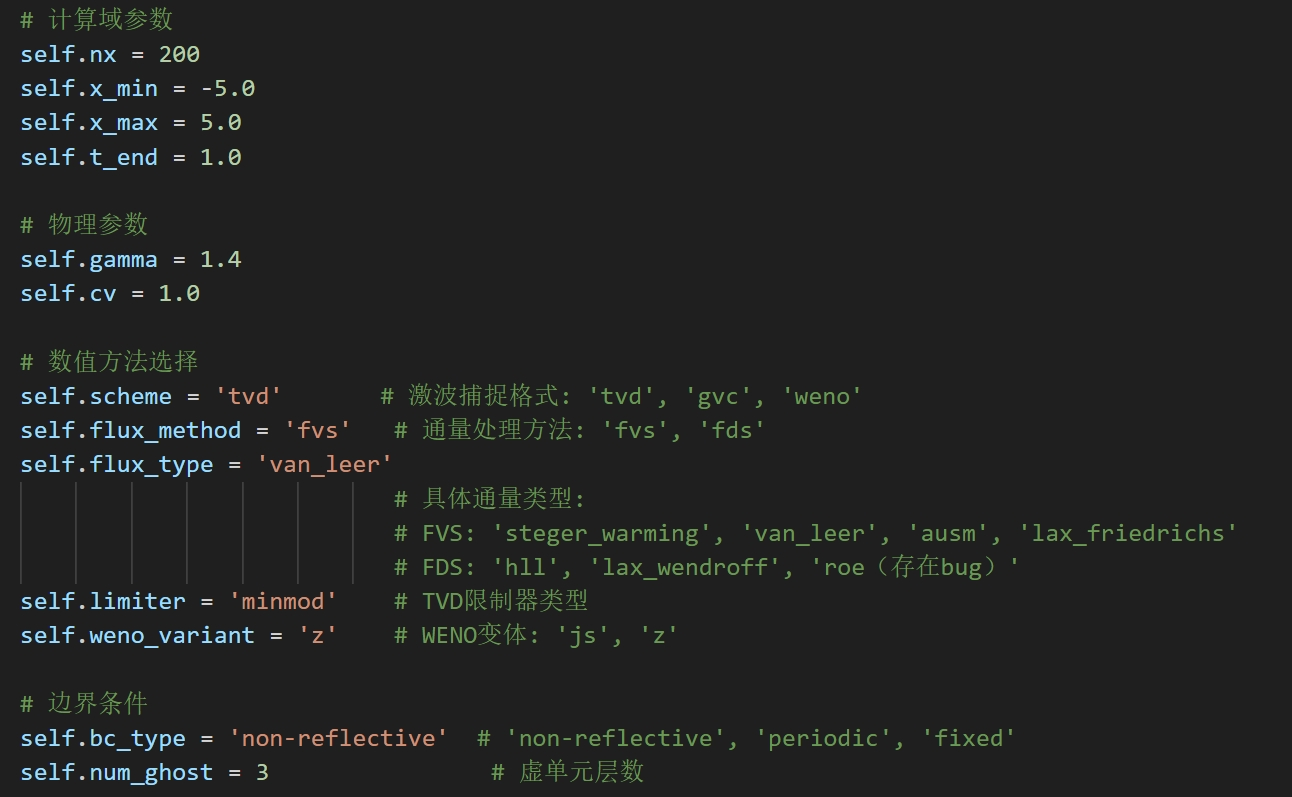
\includegraphics[width=0.8\textwidth]{config_example.png}
    \caption{config.py 参数设置示例}
    \label{fig:config_example}
\end{figure}
%插入git commit信息
\subsection{代码提交信息}
在项目开发过程中,我使用了Git进行版本控制。以下是一些关键的提交信息
%插入图片
\begin{figure}[H]
    \centering
    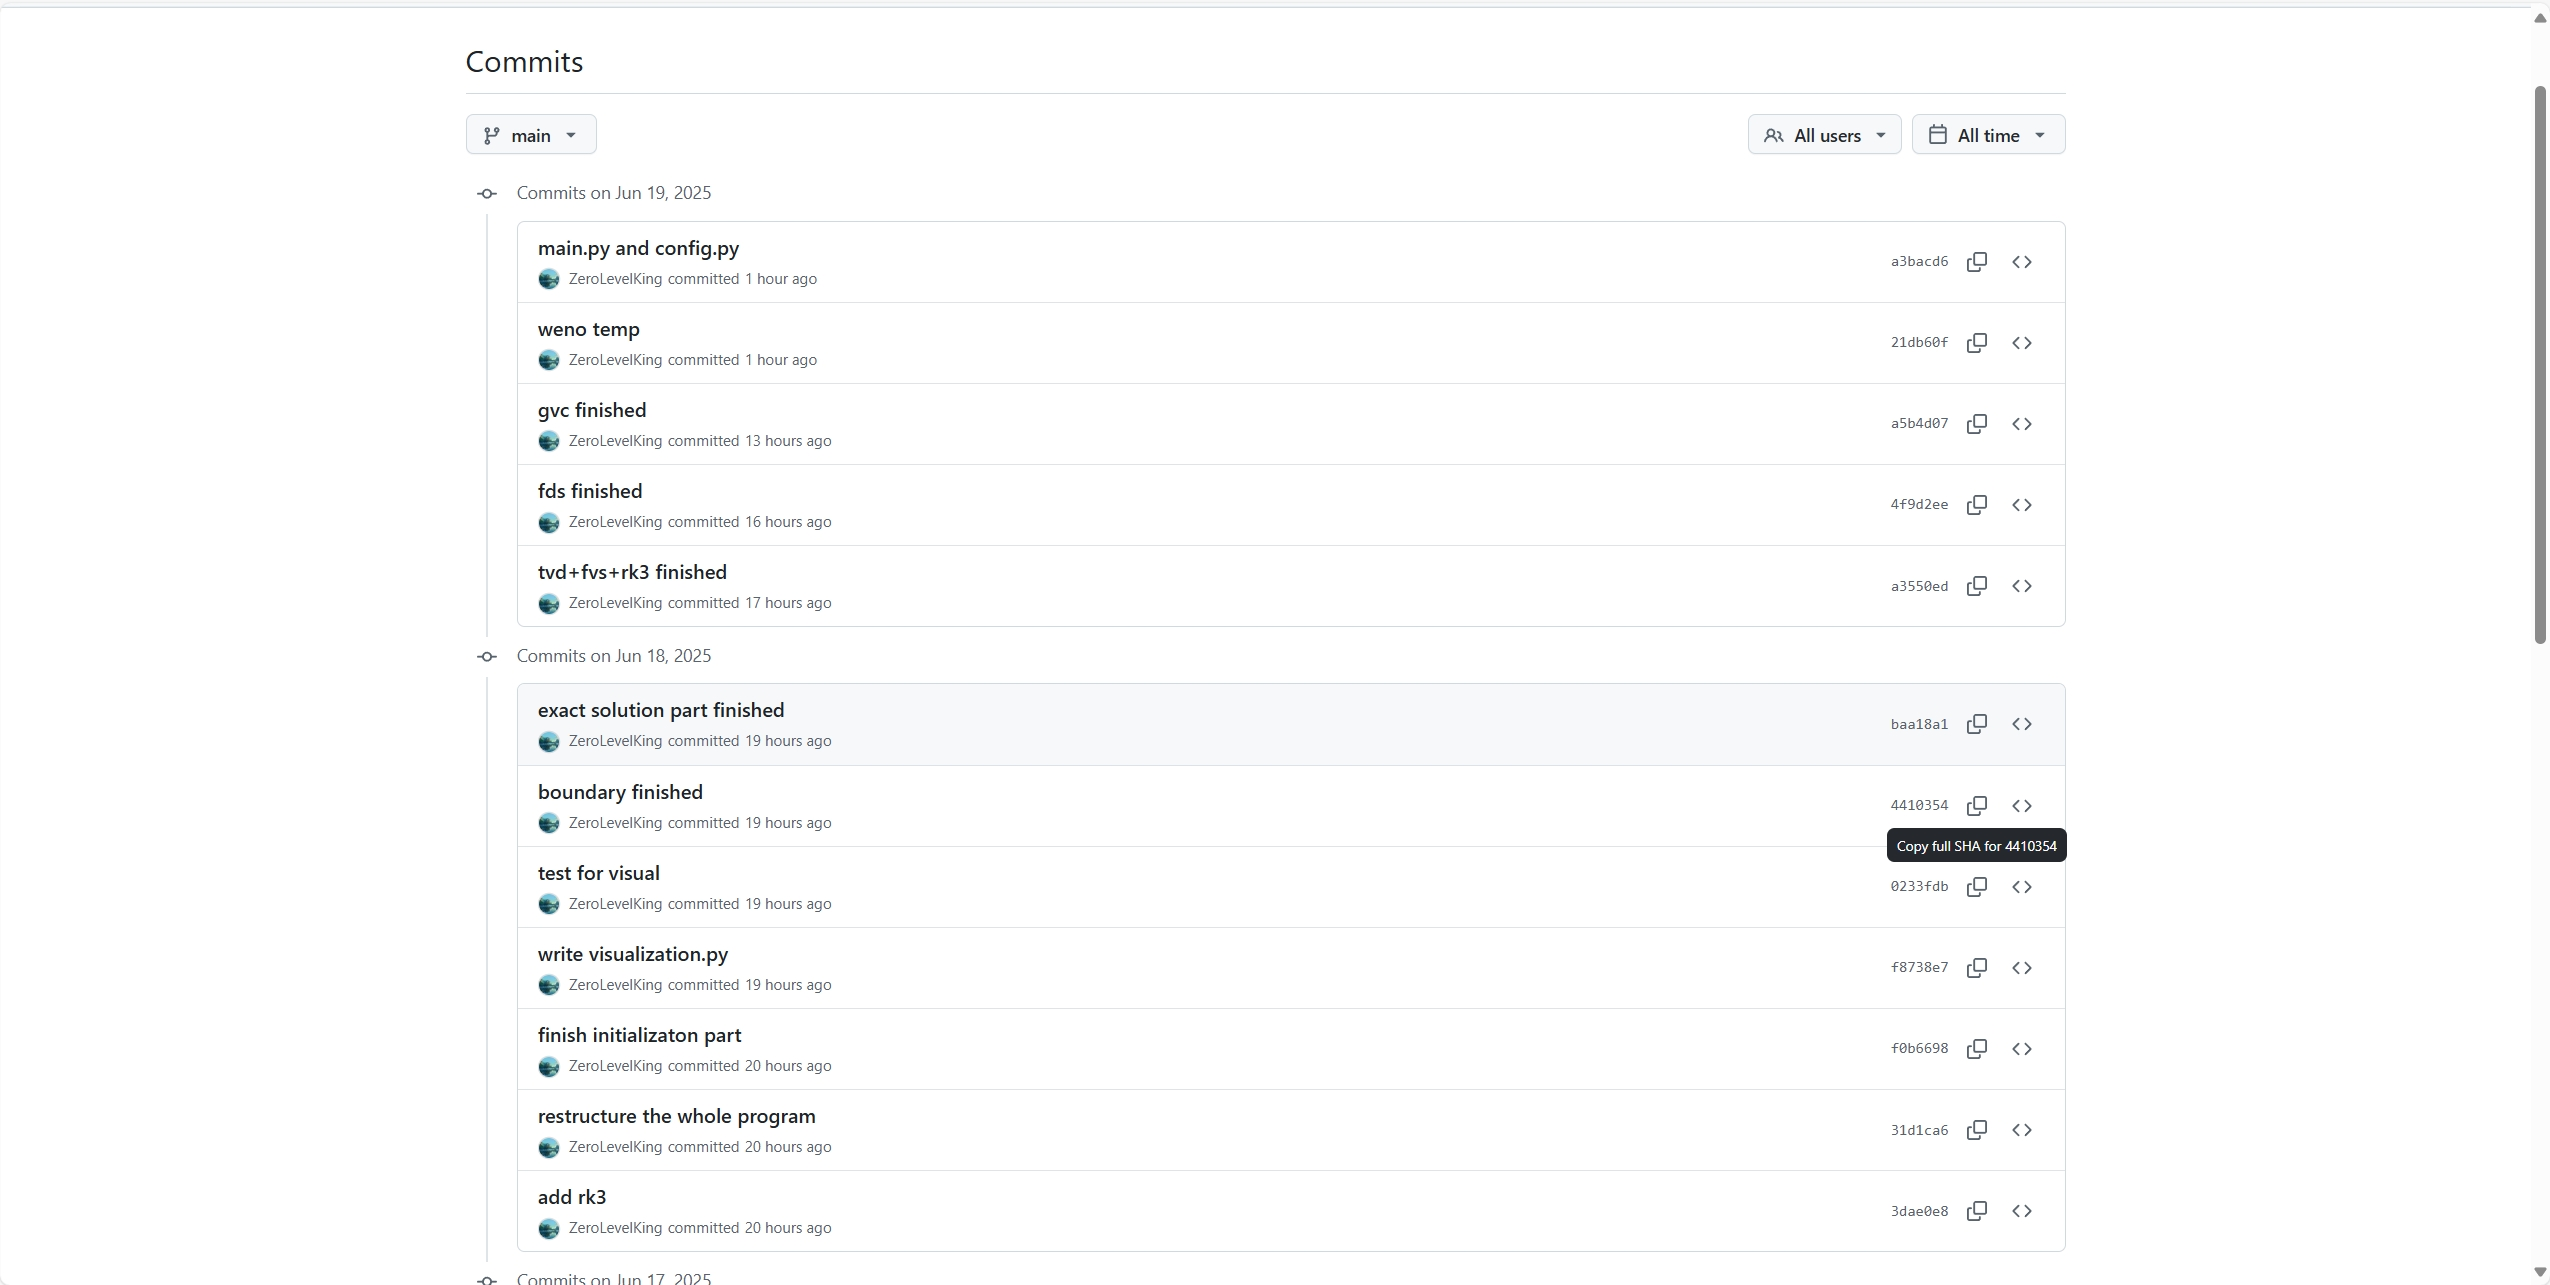
\includegraphics[width=0.8\textwidth]{c1.png}
    \caption{Git提交信息示例1}
    \label{fig:git_commit_info1}
\end{figure}
\begin{figure}
    \centering
    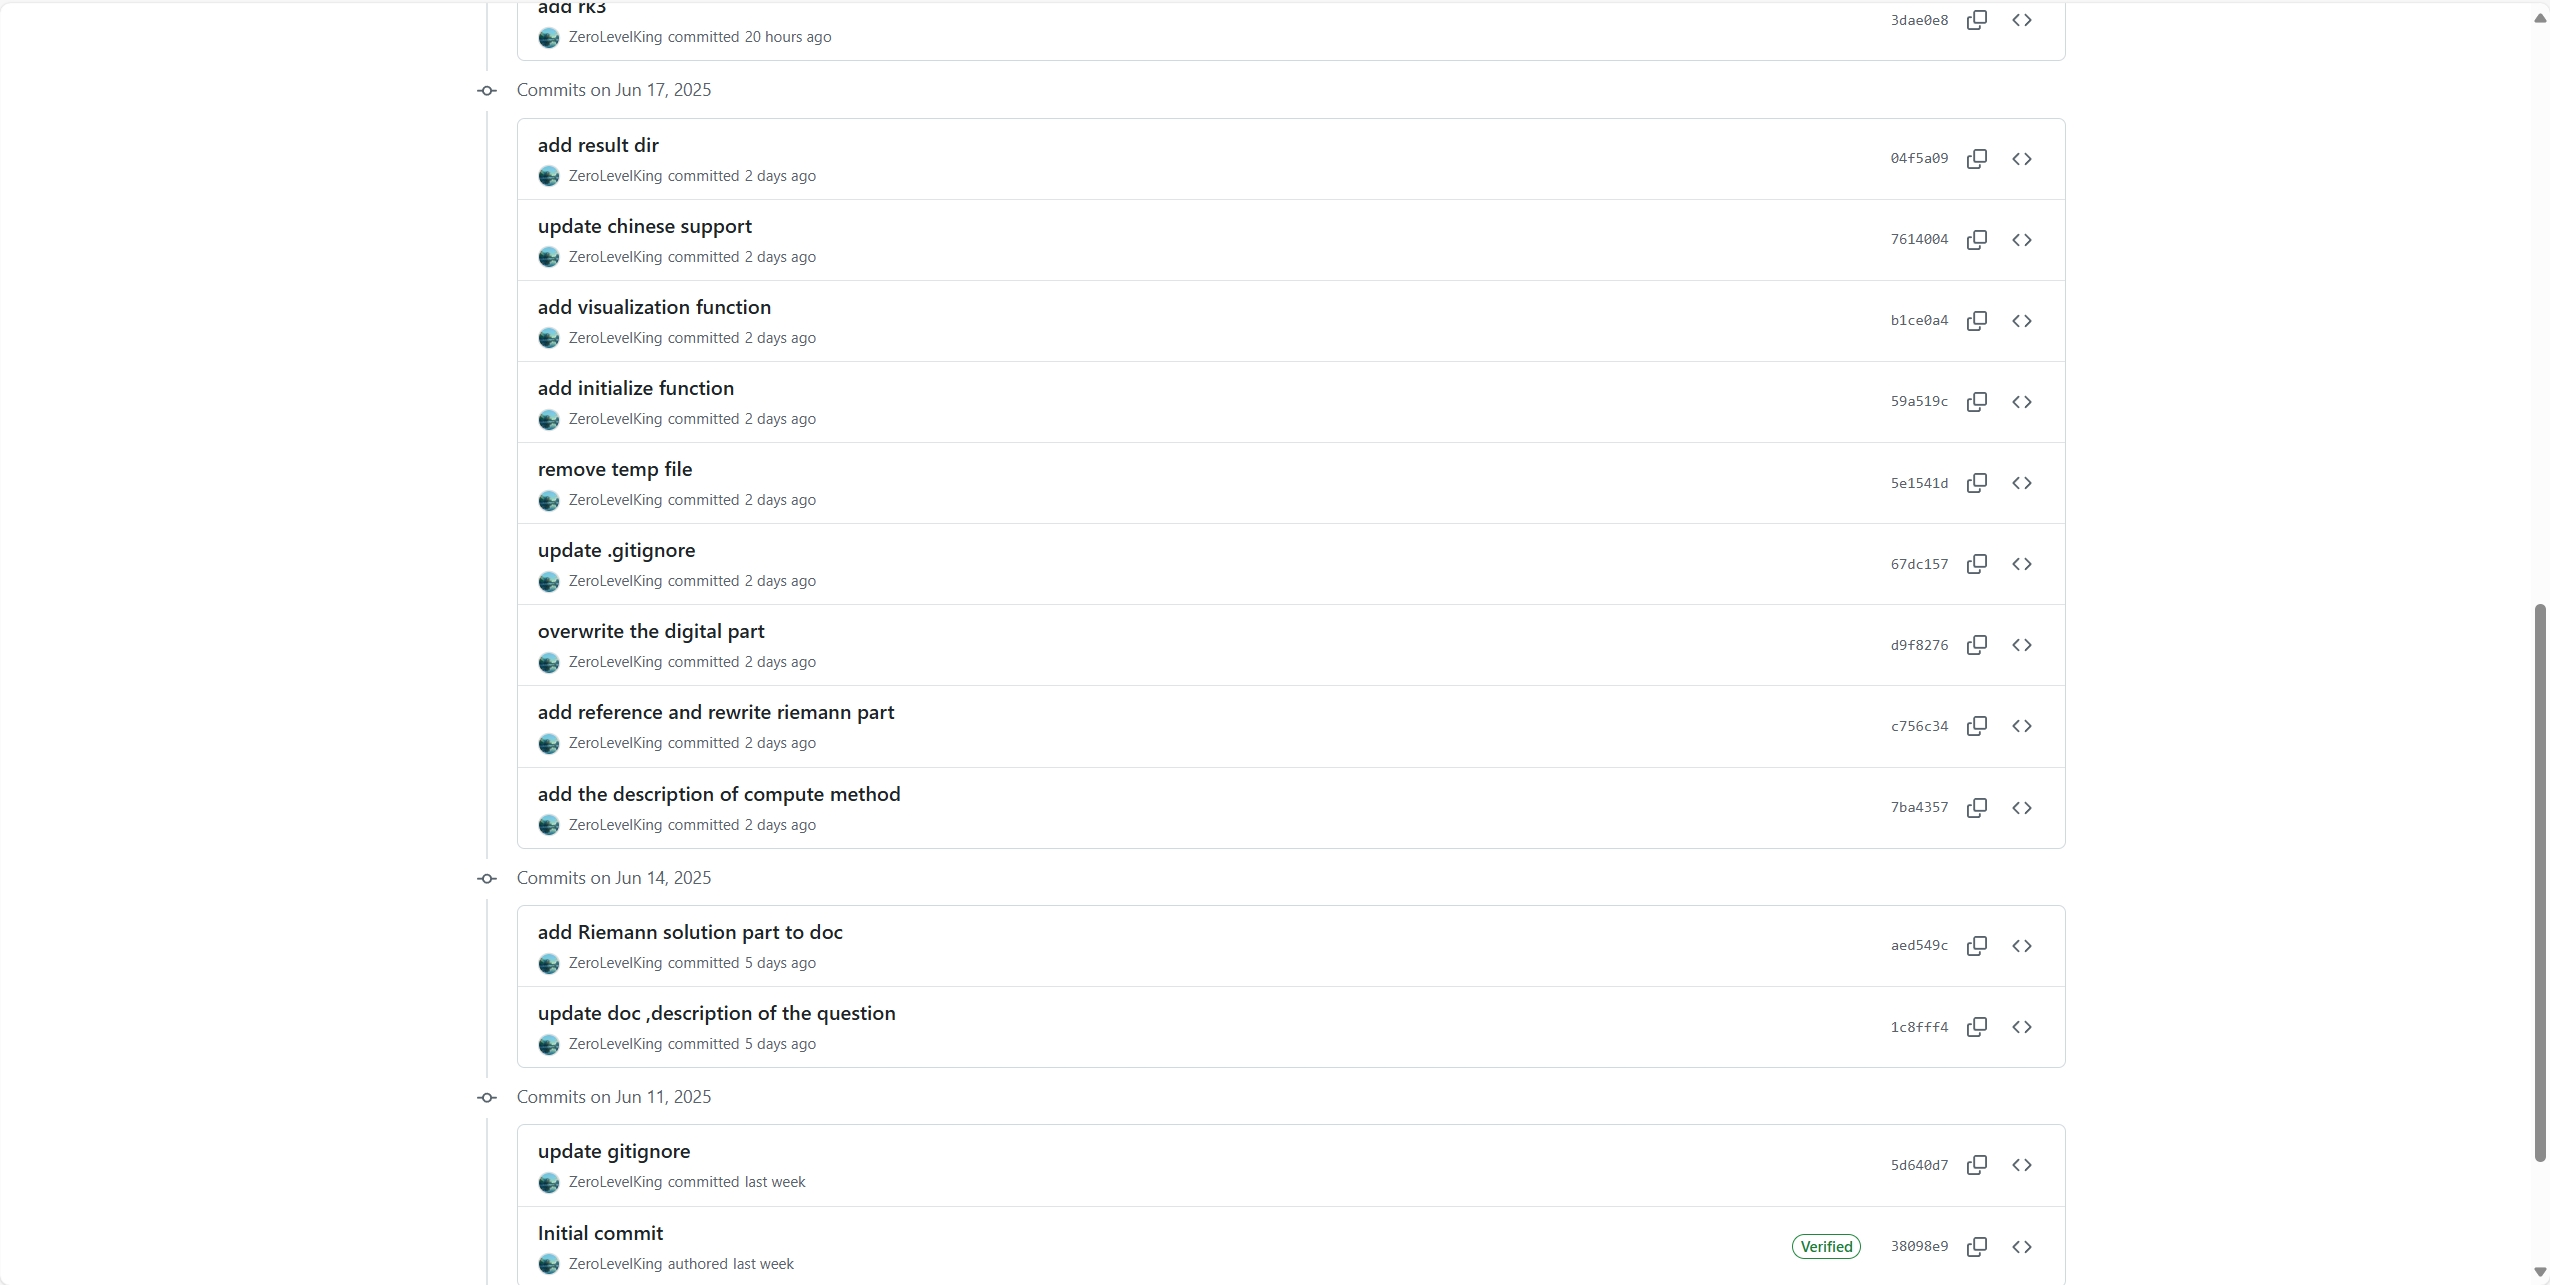
\includegraphics[width=0.8\textwidth]{c2.png}
    \caption{Git提交信息示例2}
    \label{fig:git_commit_info2}
\end{figure}


\newpage
\section{结果讨论和物理解释}



\newpage
\appendix
\section*{AI工具使用声明表}
\begin{table}[H]
    \centering
    \begin{tabular}{c|c|c}
        \hline
        使用内容 & AI工具用量 & 使用目的 \\ 
        \hline
        doc/figure/picture\_generate.py & 100\% & 使用AI生成文档中所需要的示意性图片 \\
        doc/final.tex & 20\% & 省略插入图片和写格式控制语句的重复性工作 \\ 
        ReadMe.md & 80\% & AI生成一个框架,在此基础上增加而来 \\
        .gitignore & 100\% & 针对于python和latex的自动生成.gitignore文件  \\
        src/utils/visualization.py & 30\% & 使用AI解决了中文显示问题 \\
        test/ & 90\% & 测试代码,只是调用函数,本身不涉及核心代码,用AI生成 \\
        src/ 下其余代码 & 10\% & 自己编写,用AI debug 和整理格式 \\
        \hline
    \end{tabular}
    \label{tab:AI_tools}
\end{table}


\newpage
\section*{}
% 使用标准的BibTeX格式
\bibliographystyle{unsrturl} % 更改为支持URL的样式
\bibliography{reference} % 指定BibTeX数据库文件

\end{document}